%
% path-finding
% @author Tobias Weber <tweber@ill.fr>
% @date 2021
% @license see 'LICENSE' file
%

\chapter{Path-finding Strategies}
\label{ch:paths}

This chapter develops the general theoretical idea of path-finding in a 
triple-axis spectrometer (TAS).
The path should be optimal in the sense that the instrument not only avoids 
obstacles like walls or equipment in the experimental area, but also keeps a 
maximum distance from them. 
Here, the descriptions remain ``high level'', the details and the implementation 
of the algorithm will be presented in the next chapter.

Before looking at the situation with TAS in section \ref{sec:tasrobot}, we shortly 
review the ideas of motion planning for a point-like robot in section \ref{sec:pointrobot}.



\section{Motion planning for a point-like robot}
\label{sec:pointrobot}

\subsection{Sector-based method}
\label{sec:pointrobot_sector}
An algorithm for motion planning in a point-like robot based on decomposing the 
available space into sectors is given in Ref. \cite[Ch. 13, pp. 283-306]{Berg2008}, 
whose descriptions we follow in this section. 
While the book chapter also describes polygonal robots, we limit ourselves to the 
parts that are relevant for the present work.

The movement of the point-like robot in question is not restricted to conventional 
Cartesian space, its coordinates are instead given in a general configuration space
\cite[Ch. 13.1, pp. 284-286]{Berg2008}, which more directly models its inherent 
degrees of freedom and can -- for instance -- include angular motion.

The algorithm that Berg \textit{et al.} describe consists of two parts: 
First, the separation of allowed space into sectors, within which the robot can 
move without hitting an obstacle \cite[p. 286]{Berg2008}. 
The second part concerns the computation of the actual path and is given in 
Ref. \cite[p. 289]{Berg2008}. 
In the first part, a trapezoidal map (explained below) is created for the 
configuration space containing the obstacles, both of polygonal shape. 
The trapezoids inside the obstacles are removed from the final map as the robot 
has to stay clear of them. 
The second part of the algorithm calculates the path of the robot by finding 
the trapezoids which contain the start and target point, and finding the edges 
between adjacent trapezoids from starting to ending trapezoid via a breadth-first 
search in the trapezoidal map. The robot will thus first move to the centre of 
its containing trapezoid, followed by the centre of an edge connecting the current 
to the next trapezoid, next to the centre of the next trapezoid, and so forth, 
until it arrives at its goal. 
The situation is depicted in Fig. \ref{fig:robot_trapezoids}, where we restrict 
ourselves to line-like obstacles for simplicity, effectively only using the 
second part of the algorithm.

Trapezoidal maps and the algorithm for their calculation are given in Ref. 
\cite[Ch. 6, pp. 121-146]{Berg2008}. Basically, the map of trapezoids is obtained 
by extending vertical lines from every vertex in a collection of line segments. 
The vertical extensions reach out until they intersect with another line segment 
of the collection, or an outer bounding box. The original line segment and the 
intersected segment on top (or bottom, respectively) together with the vertical 
lines form a trapezoid, as shown in Fig. \ref{fig:robot_trapezoids}. 
Together with the trapezoid map, the algorithm constructs in 
$O \left(n \log_{2} n \right)$ time a data structure, which allows querying for 
the trapezoid containing a given point with time complexity $O \left( \log_{2} n \right)$, 
where $n$ is the number of line segments \cite[Theorem 6.3, p. 133]{Berg2008}.

\begin{figure}[htb]
	\centering
	\includegraphics[width = 0.4 \textwidth]{figures/pointrobot_walls.pdf}
	\hspace{1 cm}
	\includegraphics[width = 0.4 \textwidth]{figures/pointrobot_walls_trapezoids.pdf}
	\caption[Path-finding using trapezoid maps.]{
		Left panel: A point-like robot has to find a way around line segments 
		which represent obstacles. 
		Right panel: The algorithm outlined in Ref. \cite[p. 289]{Berg2008} 
		constructs a trapezoid map and moves the robot on the shortest path from 
		the centre of one trapezoid to the centre of the edge connecting to the 
		next trapezoid, to the centre of that trapezoid, and so forth (blue arrows).}
	\label{fig:robot_trapezoids}
\end{figure}

While the present algorithm can be extended towards polygonal robots \cite[Ch. 13.3, pp. 290-297]{Berg2008} 
and provides some useful ideas, it has several severe drawbacks. First and 
foremost, the trapezoid map cannot handle the case when two or more line segment 
vertices coincide, making it very difficult to model polygonal obstacles and not 
only using mere line segments. Second, our own implementation has shown that for 
the algorithm to be stable, it has to handle many special cases, for example to 
eliminate vertices with equal $x$ coordinate components or vertical lines.

\vspace{0.5cm}

\subsection{Retraction method}
Apart from decomposing the available configuration space into sectors, a more 
direct approach can be taken. 
This approach is called the retraction method and is based on constructing the 
Voronoi regions of the obstacles and moving the robot along the Voronoi edges, 
which ensures that the path is optimal in the sense that the robot is always at 
the furthest distance from any obstacle \cite[pp. 163 and 304]{Berg2008}.
An example path for the same problem as before is given in Fig. \ref{fig:robot_voronoi}.
This approach is described in detail in \cite[pp. 247-251]{FUH_geo2020}, which 
we will follow for our TAS motion planning approach.

\begin{figure}[htb]
	\centering
	\includegraphics[width = 0.4 \textwidth]{figures/pointrobot_walls_voronoi.pdf}
	\caption[Path-finding using Voronoi diagrams.]{
		The accessible configuration space is subdivided into the Voronoi regions 
		of the obstacles (coloured). The optimal path (blue arrows) in the sense 
		that it keeps the robot at maximum distance from any obstacle, has it 
		moving along the Voronoi edges.}
	\label{fig:robot_voronoi}
\end{figure}



\section{Motion planning for a triple-axis spectrometer}
\label{sec:tasrobot}

As it is imperative that the instrument not move into any walls, we choose the 
retraction method using the obstacles' Voronoi regions.
Several coordinate systems are available for a TAS (refer to chapter \ref{ch:xtal}), 
for this reason we have got several equivalent possibilities to describe its movement. 


\subsection{Instrument positions configuration space}
The first possibility would be to model the entire instrument as a polygonal 
robot arm and directly use the position of the robot as its configuration space. 
This way it would be directly possible to use a polygonal representation of the 
walls and construct their Voronoi regions -- or even trapezoidal maps -- as 
discussed in section \ref{sec:pointrobot}. The main problem with this approach 
is the very complicated treatment that would be necessary for the instrument 
itself, as it possesses an arbitrarily complex geometry and its three axes
can move about their joints.


\subsection{Crystal coordinates configuration space}
A better way is to employ a configuration space where the instrument is represented 
as a single point in that space. 
This comes at the cost of the shape of the walls becoming more complicated when 
transformed into configuration space, they may not even be simply-connected 
any more in that space. 
There are two choices for such a configuration space: We can either use the 
reciprocal crystal coordinates as discussed in chapter \ref{ch:xtal}, or use a 
configuration space comprising the instrumental angles.
We discuss both of these cases in this and the following section.

Using the reciprocal crystal coordinates as configuration space would need a 
transformation of the walls into the four-dimensional reciprocal space 
(three momentum and on energy coordinate). Even when taking into account that 
the TAS is usually restricted to a two-dimensional scattering plane, thereby 
dropping one of the momentum dimensions, the problem would still be three-dimensional.

A typical situation is shown in Fig. \ref{fig:tas_wall} (a and b). 
Here, the instrument motion is blocked by an obstacle in the experimental zone
as well as outer walls (marked in red in panel (a)).
The crystal configuration space, panel (b), shows the allowed and forbidden
coordinates that result from the obstacles. The natural units in such a
configuration space are the relative lattice units (rlu) of the reciprocal
crystal lattice (see chapter \ref{ch:xtal}).
In the figure, the crystal configuration space seems to be simple enough for 
further consideration, but it has several disadvantages: Shown here is merely
a two-dimensional slice at $E = 0$ of the true configuration space.
Such a slice is thus not sufficient for a full analysis as the two instrument
angles that it moves are only the sample scattering and the sample crystal angle.
Of these, only the scattering angle actually moves an instrument arm, the crystal
angle is just the internal rotation on the axis.
As can be seen in Fig. \ref{fig:tas_wall} (b), the instrument cannot move
around obstacles, but is locked in isolated regions of the configuration space.
To have enough degrees of freedom for path finding, we would need to include
a third coordinate axis, the energy.
As a further negative aspect, this configuration space is dependent on the 
crystal as well as the selected scattering plane (here shown, for instance, 
is the plane spanned by the $\left[1,\,0,\,0\right]$ and $\left[0,\,1,\,0\right]$ 
vectors), so it would need to be re-calculated for every change in sample or 
scattering plane.


\subsection{Angular configuration space}
On the other hand, using the instrument angles as natural units for a configuration
space seems to be even more complicated at first glance. 
The instrument comprises six angles, namely the crystal and 
scattering angles for the monochromator, the sample and the analyser crystals, 
respectively, leading to a six-dimensional configuration space. 
When can take into account that not all angles are independent of one another:
The monochromator and analyser scattering angles are always double their 
respective crystal angles, because they both have to fulfill the Bragg condition
at all times. 
We are therefore left with four independent angles: the monochromator and analyser
scattering angles as well as the sample crystal and scattering angle. 

Furthermore, we are mainly interested in collisions of the instrument with walls 
or itself, this way the sample crystal angle can be dropped from the analysis, 
because it only rotates the sample axis, but does not move the instrument. 
It can still lead to forbidden positions if it rotates too far and rips out cables 
or tubes, but these cases we can treat as their own one-dimensional problem. 

A further simplification is possible when taking into account that during a 
typical experiment the instrument usually only moves either its monochromator 
or analyser angle to choose the energy transfer, but not both. 
Therefore, one of these angles, usually the analyser angle, rests at a constant 
value. In total, we are left with a two-dimensional configuration space composed 
of the monochromator and the sample scattering angle. 
A typical situation is shown in Fig. \ref{fig:tas_wall} (a and c). 
As before, the instrument motion is blocked by an obstacle in the experimental zone. 
The angular configuration space image, panel (c), shows that the obstacle 
transforms into a non-primitive geometric object in configuration space, 
which -- as already mentioned -- does not even have to be simply-connected.

\begin{figure}[htb]
	\centering
	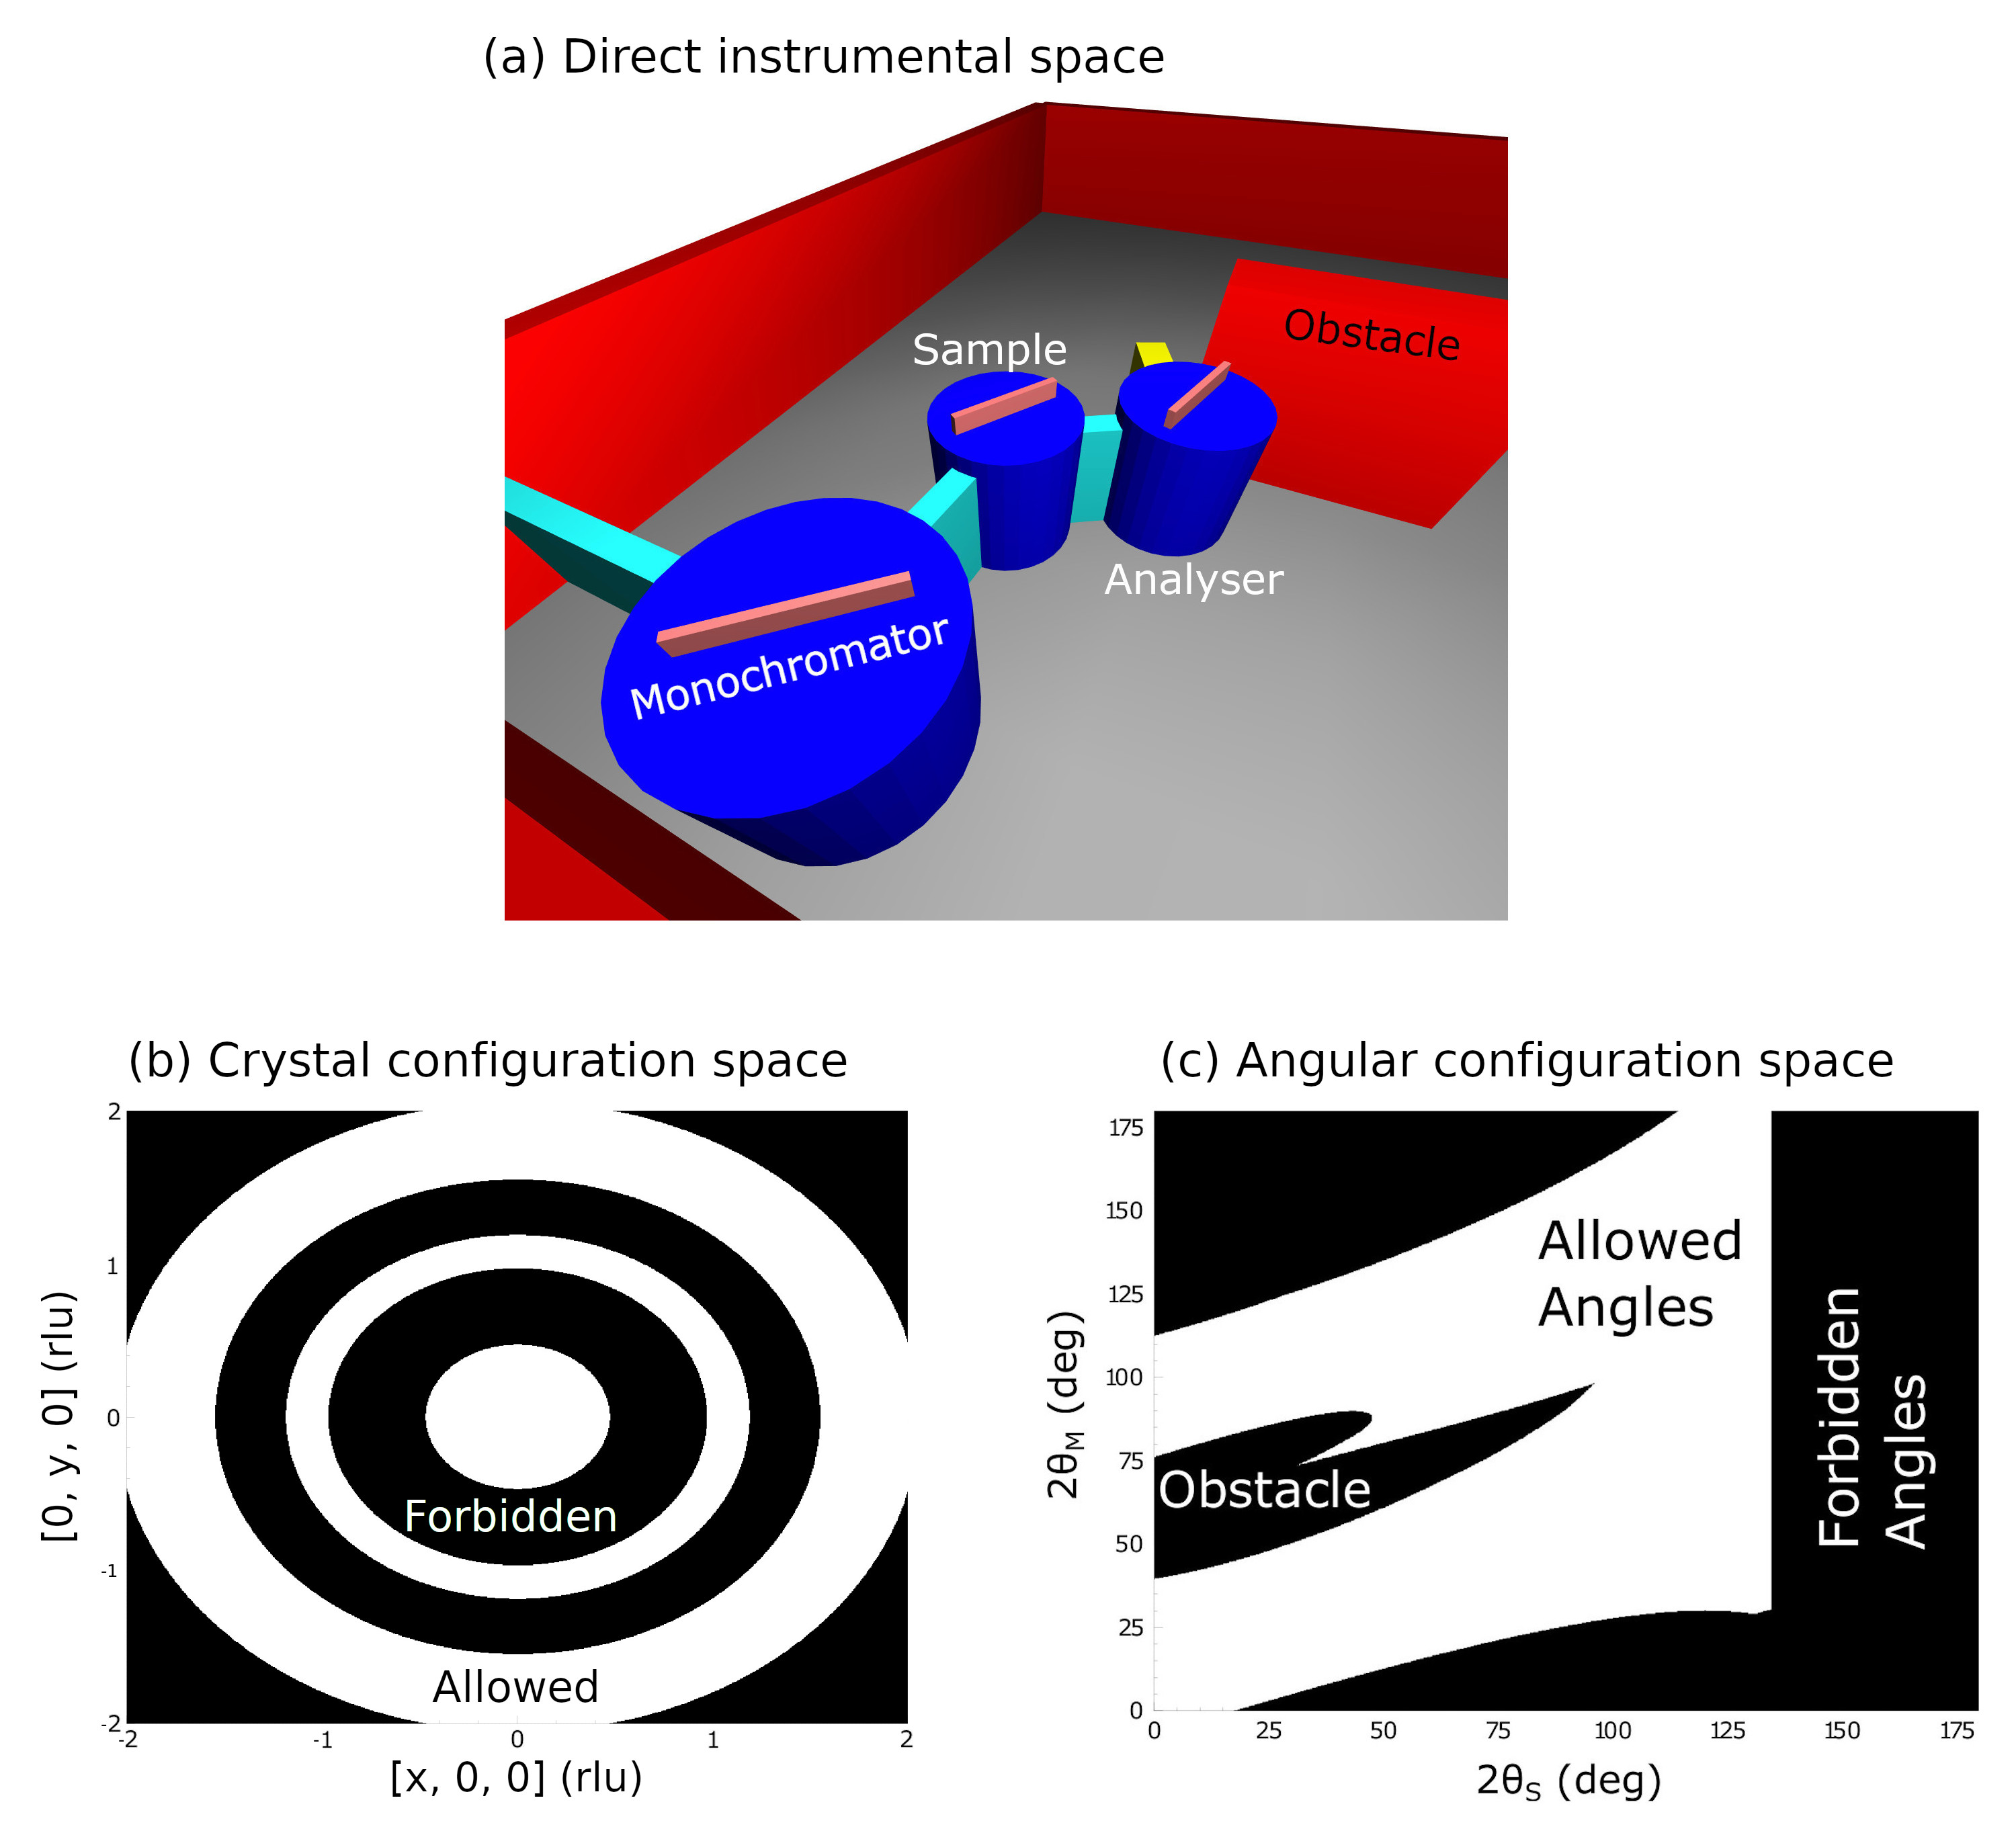
\includegraphics[width = 0.95 \textwidth]{figures/tas_wall.jpg}
	\caption[TAS configuration spaces.]{
		An obstacle as it appears in direct instrument space (a), in the 
		crystal coordinate configuration space (b) as well as the angular
		configuration space (c).
		In the configuration spaces, allowed instrument positions are 
		shown in white, forbidden positions in black. 
		The areas of disallowed positions are given either by collisions 
		of the instrument with the outer walls or with itself.}
	\label{fig:tas_wall}
\end{figure}


\subsection{Overall strategy}
\label{sec:strategy}

The strategy for planning the motion of the spectrometer comprises several steps. 
Modifying the algorithm for a point-like robot described in Ref. 
\cite[Ch. 13, pp. 283-306]{Berg2008} (see section \ref{sec:pointrobot}) and the 
retraction algorithm for finding a path using line-segment Voronoi diagrams as 
presented in \cite[p. 163]{Berg2008} and \cite[pp. 247-251]{FUH_geo2020}, we 
summarise the steps here before describing them in detail together with the actual
implementation in the next chapter.

Two tasks are needed. The first task is building the mesh of possible paths the 
instrument can move along. 
The second task concerns finding one specific path on the path mesh and moving
the instrument on that path. 
Splitting the work into a pre-built path mesh that can be used for live calculations
is an approach that is commonly used in path-finding problems \cite{Hwang2003}.
The two tasks comprise these following steps:
\begin{enumerate}
	\item Building the path mesh.
	\begin{enumerate}
		\item Calculate the angular configuration space as described above.
		\item Create a spatial index tree of the angular position of the obstacles.
			This step is needed so that we can quickly determine the distance to
			the next wall from any angular coordinate, for instance in the cost
			function for the edge weights that will be discussed in the next chapter.
		\item Trace the obstacle contours in angular configuration space. 
			This step is necessary because they can be of arbitrary
			shape in this representation and are not necessarily geometric 
			primitives, as seen in Fig. \ref{fig:tas_wall}.
		\item Approximate the traced contour curves with line segments.
		\item Simplify the line segments. This is necessary because the line 
			segments generated in the previous step are not optimal:
			First, they may contain back-to-back collinear lines which can be 
			unified. Second, jagged edges and zigzag lines may be
			produced in practice. These need to be eliminated or at least smoothed 
			before the next step.
		\item Split all polygonal line segments that build up the contours into 
			convex regions. With this we can group all lines in a convex region 
			and only calculate the Voronoi diagrams for these groups instead of 
			all line segments.
		\item Calculate the Voronoi diagram for the line segment groups. 
			The Voronoi edges are the possible instrument paths in configuration 
			space. Save both the Voronoi diagram as well as its representation 
			in a graph structure, as in \cite[p. 163]{Berg2008}.
			For quick access to the closest positions, the positions of the
			Voronoi vertices are additionally saved in a spatial index tree such as a 
			k-d tree \cite{TODO}, an R-tree \cite{TODO} or a BSP tree. 
			Please refer to chapter \ref{sec:indextrees} for a description of these data types.
			Such an approach is, for instance, used in the work by 
			Hwang \textit{et al}. \cite{Hwang2003}.
		\item Simplify the Voronoi diagram. For example, Voronoi vertices and 
			edges inside obstacle regions have to be removed.
			These are generated in the previous step because, there, no 
			differentiation was made between the ``inside'' and ``outside'' 
			regions of the convex line segment contour groups.
	\end{enumerate}

	\item Finding the instrument path and executing its motion, this is the 
		point-like limiting case of the algorithm in \cite[p. 163]{Berg2008}.
	\begin{enumerate}
		\item The user of a triple-axis spectrometer usually enters the coordinates 
			in the crystal coordinate system (see chapter \ref{ch:xtal}). The start 
			and end point of the instrument path have to be converted from crystal
			coordinates into instrument angles. The instrument angles form a 
			coordinate point in angular configuration space.
		\item Determine the Voronoi regions of the start and end coordinate points
			using the spatial index tree that was generated during the creation
			of the path mesh.
		\item Move the instrument to the edge of the start Voronoi region.
		\item Calculate a path to the edge of the Voronoi region 
			containing the end point and move the instrument along that path. 
			The path has to minimise a given cost function, which can,
			for example, lead to the shortest path or the path furthest from
			all walls. 
			In either case, Dijkstra's algorithm \cite{wiki_dijkstra}
			will be employed to get a path with minimum edge weights.
			It is the obvious choice, as Dijkstra's algorithm or an algorithm based 
			on it are commonly used in literature \cite{Hwang2003, Singal2014} 
			for such a task.
		\item Move the instrument from the edge of the Voronoi region containing 
			the end point towards that point.
	\end{enumerate}
\end{enumerate}


\section{Summary}
Different approaches to path-finding for a robotic system were discussed in this chapter.
The best strategy to the problem at hand is a Voronoi-diagram based construction of
a mesh of possible paths and an application of the classic Dijkstra algorithm for 
finding a specific path on the mesh.
An algorithm for such a task was introduced on a very general level.
Describing the details of this algorithm together with an implementation in C++  
will be left to the next chapter.
